\documentclass[11pt]{article}

% Language setting
\usepackage[turkish]{babel}
\usepackage{pythonhighlight}

\usepackage[a4paper,top=2cm,bottom=2cm,left=2cm,right=2cm,marginparwidth=2cm]{geometry}

% Useful packages
\usepackage{amsmath}
\usepackage{graphicx}
\usepackage[colorlinks=true, allcolors=blue]{hyperref}
\usepackage{verbatim}
\usepackage{fancyhdr} % for header and footer
\usepackage{titlesec}
\usepackage{parskip}

\setlength{\parindent}{0pt}

\titleformat{\subsection}[runin]{\bfseries}{\thesubsection}{1em}{}

\pagestyle{fancy} % activate the custom header/footer

% define the header/footer contents
\lhead{\small{23BLM-4014 Yapay Sinir Ağları Ara Sınav Soru ve Cevap Kağıdı}}
\rhead{\small{Dr. Ulya Bayram}}
\lfoot{}
\rfoot{}

% remove header/footer on first page
\fancypagestyle{firstpage}{
  \lhead{}
  \rhead{}
  \lfoot{}
  \rfoot{\thepage}
}
 

\title{Çanakkale Onsekiz Mart Üniversitesi, Mühendislik Fakültesi, Bilgisayar Mühendisliği Akademik Dönem 2022-2023\\
Ders: BLM-4014 Yapay Sinir Ağları/Bahar Dönemi\\ 
ARA SINAV SORU VE CEVAP KAĞIDI\\
Dersi Veren Öğretim Elemanı: Dr. Öğretim Üyesi Ulya Bayram}
\author{%
\begin{minipage}{\textwidth}
\raggedright
Öğrenci Adı Soyadı: Aybüke Sümeyye Kaçar\\ % Adınızı soyadınızı ve öğrenci numaranızı noktaların yerine yazın
Öğrenci No: 190401035
\end{minipage}%
}

\date{14 Nisan 2023}

\begin{document}
\maketitle

\vspace{-.5in}
\section*{Açıklamalar:}
\begin{itemize}
    \item Vizeyi çözüp, üzerinde aynı sorular, sizin cevaplar ve sonuçlar olan versiyonunu bu formatta PDF olarak, Teams üzerinden açtığım assignment kısmına yüklemeniz gerekiyor. Bu bahsi geçen PDF'i oluşturmak için LaTeX kullandıysanız, tex dosyasının da yer aldığı Github linkini de ödevin en başına (aşağı url olarak) eklerseniz bonus 5 Puan! (Tavsiye: Overleaf)
    \item Çözümlerde ya da çözümlerin kontrolünü yapmada internetten faydalanmak, ChatGPT gibi servisleri kullanmak serbest. Fakat, herkesin çözümü kendi emeğinden oluşmak zorunda. Çözümlerinizi, cevaplarınızı aşağıda belirttiğim tarih ve saate kadar kimseyle paylaşmayınız. 
    \item Kopyayı önlemek için Github repository'lerinizin hiçbirini \textbf{14 Nisan 2023, saat 15:00'a kadar halka açık (public) yapmayınız!} (Assignment son yükleme saati 13:00 ama internet bağlantısı sorunları olabilir diye en fazla ekstra 2 saat daha vaktiniz var. \textbf{Fakat 13:00 - 15:00 arası yüklemelerden -5 puan!}
    \item Ek puan almak için sağlayacağınız tüm Github repository'lerini \textbf{en geç 15 Nisan 2023 15:00'da halka açık (public) yapmış olun linklerden puan alabilmek için!}
    \item \textbf{14 Nisan 2023, saat 15:00'dan sonra gönderilen vizeler değerlendirilmeye alınmayacak, vize notu olarak 0 (sıfır) verilecektir!} Son anda internet bağlantısı gibi sebeplerden sıfır almayı önlemek için assignment kısmından ara ara çözümlerinizi yükleyebilirsiniz yedekleme için. Verilen son tarih/saatte (14 Nisan 2023, saat 15:00) sistemdeki en son yüklü PDF geçerli olacak.
    \item Çözümlerin ve kodların size ait ve özgün olup olmadığını kontrol eden bir algoritma kullanılacaktır. Kopya çektiği belirlenen vizeler otomatikman 0 (sıfır) alacaktır. Bu nedenle çözümlerinizi ve kodlarınızı yukarıda sağladığım gün ve saatlere kadar kimseyle paylaşmayınız.
    \item Bu vizeden alınabilecek en yüksek not 100'dür. Toplam aldığınız puan 100'ü geçerse, aldığınız not 100'e sabitlenecektir.
    \item LaTeX kullanarak PDF oluşturanlar öz geçmişlerine LaTeX bildiklerini de eklemeyi unutmasınlar :)
    \item Bu vizedeki soruların çözümleri ve tex dosyası için istediğiniz kadar sayıda Github repository'si oluşturabilirsiniz. Sadece yukarıda belirttiğim tarihlerde (14 Nisan 2023 saat 15:00 ile 15 Nisan 2023 saat 15:00 arasında) public yapmayı/halka açmayı ve Github profilinizi de öz geçmişinize eklemeyi unutmayın :)
    \item Bilgisayarınıza hiçbir program kurmadan, Overleaf, Google Colab, Kaggle gibi ortamlar üzerinden bu vizeyi tamamlamanız mümkün. İyi çalışmalar!!
\end{itemize}

(Ekstra 5 puan) \url{https://github.com/aybukekcr/VizeTex}

\newpage
\section{(Toplam 10 Puan) Hopfield Networks:}

\subsection{(2 Puan)} \textbf{ChatGPT’ye size Hopfield Network’ler ile ilgili detaylı bilgi vermesini isteyin. Sorduğunuz soruyu, ChatGPT'nin çıkartığı cevabı aşağı koyun. Bu cevapta anlamadığınız terimleri de ChatGPT’ye sorup, sorduğunuz soruları ve ChatGPT’nin verdiği cevapları da sırayla aşağı koyun.}

Hopfield Network'ler ile ilgili detaylı bilgi verebilir misin?
Elman Hopfield tarafından 1982 yılında tanıtılan Hopfield Ağı, birçok alanda kullanılan bir yapay sinir ağı türüdür. Bu ağ, bağlantılı bir ağdır ve düğümleri (nöronları) her biri iki durumlu (etkin ve etkisiz) olan bir ağdır. Bu nöronlar, her biri diğer nöronlarla bağlantılıdır ve her bir bağlantının gücü belirli bir ağırlıkla belirtilir.
Hopfield ağları, özellikle en çok hatırlama (recall) işlemleri için kullanılır. Bu ağ, önceden belirtilen bir deseni hatırlamak için kullanılır ve deseni yeniden oluşturmak için kullanılabilir. Bu nedenle, sınıflandırma veya tanıma için kullanılmaz.
Hopfield ağları, nöronlar arasındaki bağlantılar sayesinde hafızayı ve hatırlamayı sağlar. Ağdaki her nöron, diğer nöronların durumunu ve ağırlıklarını hesaba katarak kendi durumunu belirler. Aynı zamanda, ağ toplam enerjisi en düşük seviyede tutulur ve ağdaki nöronların durumu bu enerji seviyesine bağlı olarak değişir.
Hopfield ağları, biyolojik nöronların davranışlarını taklit etmeye çalışır ve aynı zamanda bellek, tanıma ve düzenleme gibi problemleri çözmek için kullanılır. Bu ağlar, elektriksel sinyallerin nasıl etkileşime girdiğini hesaplar ve her nöronun çıkışını hesaplayarak ağdaki tüm nöronların durumunu belirler.

Etkin ve etkisiz durum nedir?

Hopfield ağlarında, nöronlar iki durumlu olabilirler: etkin (aktif) veya etkisiz (pasif). Etkin durumda olan bir nöron, diğer nöronlarla bağlantılı olan nöronlar tarafından etkilenir ve kendi durumunu günceller. Etkisiz durumda olan bir nöron ise diğer nöronları etkilemez ve ağda bir rolü yoktur.

Bu iki durum genellikle +1 ve -1 olarak ifade edilir. Etkin durum +1 olarak ifade edilirken, etkisiz durum -1 olarak ifade edilir. Bu nedenle, bir nöronun etkin veya etkisiz durumu, nöronun çıkışının +1 veya -1 olmasına bağlıdır.

Ağ toplam enerjisi nedir ?

Hopfield ağlarında, ağın toplam enerjisi, tüm nöronların bağlantılarındaki ağırlıkların ve nöronların etkinlik durumlarının bir fonksiyonudur. Toplam enerji, ağdaki tüm nöronların durumlarına göre hesaplanır ve enerjinin düşük seviyede kalması amaçlanır. Ağın toplam enerjisi, ağın hatırlama (recall) yeteneği ile yakından ilişkilidir ve enerjinin en düşük seviyede kalması, ağın kararlılığı ve doğru hatırlama yapabilmesi için önemlidir.


\subsection{(8 Puan)} \textbf{ChatGPT’nin açıklamalarından ne anladığınızı buraya kendi kelimelerinizle özetleyin. Örneğin ``Hopfield Network nedir? Ne işe yarar? Neden bilmemiz gerekir bunu? Gerçek hayatta kullanılıyor mu?'' gibi. Anlamadığınız kısımlar varsa ve ChatGPT’nin açıklamaları yeterli gelmezse internet dahil farklı kaynaklardan araştırıp, bilgilerin doğruluğunu sorgulamakta serbestsiniz. Konuyu doğru anlayıp anlamamanız puana etki edecektir. Kullandığınız kaynakları da belirtin!}

Hopfield network, biyolojik nöronların davranışlarını taklit etmeye çalışan bir yapay sinir ağı türüdür. Genellikle daha önceden verilen bir deseni hatırlama ve yeniden oluşturmak için kullanılır. Bellek işlevi, tanıma ve hatırlama için de kullanılır. 
Hatırlamayı nöronlar arasındaki bağlantılar sayesinde sağlar. Birbirine bağlı bir dizi nöronla oluştuğundan bağlantılı networklerdir. Her nöron bir input alır ve output üretir. Nöronları iki durumludur, etkin ve etksiz olabilir. Etkin nöronlar diğer nöronlar diğer nöronlarla bağlantılı nöronlardan etkilenir. Etkisiz nöronların ise ağda bir rolü yoktur.
Ağın kararlılığı ve doğru hatırlama yapabilmesi için ağ toplam enerjisinin en düşük seviyede kalması gerekir. Ağ toplam enerjisi, tüm nöronların durumlarına göre hesaplanır.
Nöron sayısının artmasıyla ağın karmaşıklığı artacağından daha büyük ve karmaşık problemleri çözebilir. 
Şifreleme işlemlerinde, bozuk şekillerin yeniden oluşturulmasında, el yazı tanımlama sistemlerinde, parmak izi okumada kullanılır.
Gerçek hayatta uygulanabilir olduğundan ve yapay zeka teknolojilerinin nasıl işlediğini anlamamız için önemlidir.

\url{https://medium.com/@batincangurbuz/hopfield-a%C4%9F-modeli-hopfield-network-hn-ccf1548ca432}


\section{(Toplam 10 Puan) Boltzman Machine:}

\subsection{(2 Puan)} \textbf{ChatGPT’ye size Boltzman Machine ilgili detaylı bilgi vermesini isteyin. Sorduğunuz soruyu, ChatGPT'nin çıkartığı cevabı aşağı koyun. Bu cevapta anlamadığınız terimleri de ChatGPT’ye sorup, sorduğunuz soruları ve ChatGPT’nin verdiği cevapları da sırayla aşağı koyun.}

Boltzman Machine hakkında detaylı bilgi verir misin? 
Boltzmann Machine bir tür yapay sinir ağıdır ve karmaşık desenleri modellemek ve öğrenmek için olasılıksal yöntemler kullanır. Boltzmann Machine, 1980'lerin başında Geoffrey Hinton ve Terry Sejnowski tarafından icat edildi ve daha sonra derin öğrenme modellerinde yaygın olarak kullanıldı.

Boltzmann Machine, birbirine bağlı ağırlıklar aracılığıyla bağlanan bir dizi düğümden veya nörondan oluşur. Ağdaki her düğüm, "açık" veya "kapalı" olmak üzere iki durumdan birinde olabilir. Her düğüm, diğer düğümlere bağlanan ağırlıkları ile etkileşime girer ve her bir düğümün durumunu belirleyen bir aktivasyon işlevine sahiptir.

Bir Boltzmann Machine, iki tür düğüme sahiptir: görünür ve gizli. Görünür düğümler, ağa verilen girdi verilerini temsil ederken, gizli düğümler, görünür düğümlerle bağlantılı olarak öğrenilen gizli desenleri temsil eder. Bu özellikleri sayesinde Boltzmann Machine, girdilerdeki desenleri algılamayı öğrenir ve verilen bir girdi verisiyle ilişkili olasılık dağılımını tahmin etmek için kullanılabilir.

Bir Boltzmann Machine, bir enerji fonksiyonu kullanır. Bu enerji fonksiyonu, ağırlıkların ve düğümlerin durumlarına göre hesaplanır. Ağın öğrenmesi, enerji fonksiyonunun minimize edilmesine dayanır. Bu minimize edilmiş enerji fonksiyonu, ağın öğrendiği modelin kalitesini belirler.

Boltzmann Machine, özellikle öznitelik çıkarımı, veri sıkıştırma ve sinir ağı modellerinin oluşturulması gibi birçok uygulama için kullanılabilir. Ancak, ağın eğitimi, hesaplama açısından maliyetlidir ve daha sonraki derin öğrenme tekniklerinin geliştirilmesiyle bazı dezavantajları ortaya çıkmıştır.

Düğümlerin açık ve kapalı olması nedir?

Bir düğümün açık veya kapalı olması, Boltzmann Machine'de kullanılan iki durumdan biridir. Bu durum, bir düğümün aktivasyon seviyesini ifade eder.

Bir düğümün açık olması, aktivasyon seviyesinin yüksek olduğu anlamına gelir. Bu, o düğümün etkin olduğunu ve ağdaki işlemlere katıldığını gösterir. Öte yandan, bir düğümün kapalı olması, aktivasyon seviyesinin düşük olduğu anlamına gelir. Bu, o düğümün etkin olmadığını ve ağdaki işlemlere katılmadığını gösterir.

Boltzmann Machine'de, açık ve kapalı durumlar, ağdaki her bir düğümün durumunu temsil eder. Bu durumlar, ağın veriye veya modele göre öğrenme yapabilmesini sağlar. Ayrıca, bu durumlar, veri analizi ve modelleme için kullanılan olasılık hesaplamalarında önemlidir.



\subsection{(8 Puan)} \textbf{ChatGPT’nin açıklamalarından ne anladığınızı buraya kendi kelimelerinizle özetleyin. Örneğin ``Boltzman Machine nedir? Ne işe yarar? Neden bilmemiz gerekir bunu? Gerçek hayatta kullanılıyor mu?'' gibi. Anlamadığınız kısımlar varsa ve ChatGPT’nin açıklamaları yeterli gelmezse internet dahil farklı kaynaklardan araştırıp, bilgilerin doğruluğunu sorgulamakta serbestsiniz. Konuyu doğru anlayıp anlamamanız puana etki edecektir. Kullandığınız kaynakları da belirtin!}

Boltzman machine karmaşık desenleri modellemek ve öğrenmek için kullanılan bir yapay sinir ağıdır. Modelleme ve öğrenme için olasılıksal yöntemler kullanır. Bir çok gizli katmana sahiptir. Girdi verilerinin analiz edilmesi, modellemesi, veriler arasındaki ilişkilerin anlaşılması ve sonrasında tahmin ve sınıflandırma yapılması için kullanılır. Çıktıları hesaplamak için her bir düğümün durumunu, ağın toplam enerjisini hesaplar. Daha sonra ağ veriler arasındaki bağlantıları öğrenmek ve verileri analiz etmek için bir öğrenme süreci başlatır. Öğrenme sürecinde iki tür düğüm kullanılır: görünür ve gizli düğümler. Görünür düğümler, ağa dışarıdan gelen verileri temsil eder, gizli düğümler ağın içindedir ve verilerin özelliklerini temsil eder. Ağın öğrendiği modelin kalitesini enerji fonksiyonu belirler. Enerji fonksiyonu minimize edilmelidir.
Boltzman machine, veri analizi ve modelleme, öznitelik çıkarımı, veri sıkıştırma için kullanılabilir. Eğitim için hesaplama açısından maliyetlidir ve bazı dezavatajları vardır. Bu nedenle yeni derin öğrenme teknikleri ve sinir ağı modelleri geliştirilmiştir.
Yapay zeka alanındaki öğrenme ve modelleme süreçlerinde kullanılan temel kavramlar ve tekniklerin anlaşılması için de önemlidir. 
Görüntü işleme, NLP öneri sistemleri gibi uygulamalarda çok kullanılır. Netflix, amazon, youtube gibi kişiye özel içerik sunan platformlarda, hastalık tahmini için tıbbi alanda, güvenliği artırmak için siber güvenlik alanında kullanılır. 


\section{(Toplam 10 Puan) Markov Assumption ve Markov Chain:}

\subsection{(2 Puan)} \textbf{ChatGPT’ye size Markov assumption ve Markov Chain ilgili detaylı bilgi vermesini isteyin. Sorduğunuz soruyu, ChatGPT'nin çıkartığı cevabı aşağı koyun. Bu cevapta anlamadığınız terimleri de ChatGPT’ye sorup, sorduğunuz soruları ve ChatGPT’nin verdiği cevapları da sırayla aşağı koyun.}

Markov Assumption ve Markov Chain hakkında detaylı bilgi verir misin?

Markov zinciri veya Markov süreci, rastgele bir sürecin, gelecekteki durumunun, sadece mevcut durumunun, geçmiş durumların bir etkisinin olmadığı bir olasılık dağılımı ile belirlendiği bir matematiksel modeldir.

Markov zincirindeki en önemli varsayım, Markov varsayımıdır. Bu varsayım, gelecekteki durumun, mevcut durumunun sadece bir fonksiyonu olduğunu söyler. Yani, gelecekteki durum, sadece mevcut durum ve geçmiş durumların değil, gelecekteki diğer durumların da bir fonksiyonu değildir.

Markov zinciri, durumların bir kümesinden ve her bir durumun belirli bir olasılıkla başka bir duruma geçiş yaptığı bir geçiş olasılığı matrisinden oluşur. Bu matris, herhangi bir zamandaki durumların olasılık dağılımını hesaplamak için kullanılabilir. Markov zinciri, birçok uygulamada kullanılır, örneğin doğal dil işleme, finansal piyasalar ve fiziksel sistemler gibi alanlarda.

Markov zinciri, Markov sürecinin özel bir türüdür. Markov süreci, bir sistemin sürekli zamanlı bir şekilde değiştiği, ancak herhangi bir zamandaki durumun sadece mevcut durum ve geçmiş durumların bir fonksiyonu olduğu bir olasılık sürecidir. Bu süreç, aynı zamanda Markov özelliğine sahiptir. Markov özelliği, gelecekteki durumun mevcut durumunun bir fonksiyonu olduğu fikrine dayanır.

Markov süreçleri, matematiksel modellerde ve uygulamalarda yaygın olarak kullanılmaktadır. Örneğin, birçok yapay zeka ve makine öğrenmesi algoritması, zaman serilerini modellemek için Markov süreçlerini kullanır.


\subsection{(8 Puan)} \textbf{ChatGPT’nin açıklamalarından ne anladığınızı buraya kendi kelimelerinizle özetleyin. Örneğin ``Markov assumption ve Markov Chain nedir? Ne işe yarar? Neden bilmemiz gerekir bunu? Gerçek hayatta kullanılıyor mu?'' gibi. Anlamadığınız kısımlar varsa ve ChatGPT’nin açıklamaları yeterli gelmezse internet dahil farklı kaynaklardan araştırıp, bilgilerin doğruluğunu sorgulamakta serbestsiniz. Konuyu doğru anlayıp anlamamanız puana etki edecektir. Kullandığınız kaynakları da belirtin!}

Markov assumption, bir sürecin sadece mevcut duruman bağlı olduğu ve geçmiş durumların etkisinin olmadığı varsayımıdır. Bu varsayım, Markov chain matematiksel modelinde kullanılır. 
Markov chain veya Markov süreci, belirli bir durumdan diğer durumlara geçişin dağılımlarını modellemek için kullanılır. Geçiş olasılığı matrisinden oluşur. Bu matris herhangi bir zamandaki durumların olasılık dağılımın hesaplamak için kullanılır. Markov chaindeki en önemli varsayım Markov varsayımıdır. Bu sürecin hafızasız olması en önemli özelliklerindendir. 
Markov chain ve Markov assumption, rastgele süreçlerin analizi ve modellemesi için kullanılırlar. Örnek olarak NLP, finansal piyasalar, optimizasyon problemleri, yapay zeka ve bir çok alan verilebilir. 


\section{(Toplam 20 Puan) Feed Forward:}
 
\begin{itemize}
    \item Forward propagation için, input olarak şu X matrisini verin (tensöre çevirmeyi unutmayın):\\
    $X = \begin{bmatrix}
        1 & 2 & 3\\
        4 & 5 & 6
        \end{bmatrix}$
    Satırlar veriler (sample'lar), kolonlar öznitelikler (feature'lar).
    \item Bir adet hidden layer olsun ve içinde tanh aktivasyon fonksiyonu olsun
    \item Hidden layer'da 50 nöron olsun
    \item Bir adet output layer olsun, tek nöronu olsun ve içinde sigmoid aktivasyon fonksiyonu olsun
\end{itemize}

Tanh fonksiyonu:\\
$f(x) = \frac{exp(x) - exp(-x)}{exp(x) + exp(-x)}$
\vspace{.2in}

Sigmoid fonksiyonu:\\
$f(x) = \frac{1}{1 + exp(-x)}$

\vspace{.2in}
 \textbf{Pytorch kütüphanesi ile, ama kütüphanenin hazır aktivasyon fonksiyonlarını kullanmadan, formülünü verdiğim iki aktivasyon fonksiyonunun kodunu ikinci haftada yaptığımız gibi kendiniz yazarak bu yapay sinir ağını oluşturun ve aşağıdaki üç soruya cevap verin.}
 
\subsection{(10 Puan)} \textbf{Yukarıdaki yapay sinir ağını çalıştırmadan önce pytorch için Seed değerini 1 olarak set edin, kodu aşağıdaki kod bloğuna ve altına da sonucu yapıştırın:}

% Latex'de kod koyabilirsiniz python formatında. Aşağıdaki örnekleri silip içine kendi kodunuzu koyun
\begin{python}
import torch
import torch.nn as nn

torch.manual_seed(1)

def tanh_activation(x):
    return (torch.exp(x) - torch.exp(-x)) / (torch.exp(x) + torch.exp(-x))

def sigmoid_activation(x):
    return 1 / (1 + torch.exp(-x))

X = torch.tensor([[1, 2, 3], [4, 5, 6]], dtype=torch.float32)

input_size = X.shape[1]
hidden_size = 50
output_size = 1

W1 = torch.randn(input_size, hidden_size) * 0.01
b1 = torch.zeros(hidden_size)

W2 = torch.randn(hidden_size, output_size) * 0.01
b2 = torch.zeros(output_size)

hidden_layer = tanh_activation(torch.matmul(X, W1) + b1)
output_layer = sigmoid_activation(torch.matmul(hidden_layer, W2) + b2)

print(output_layer)
\end{python}

tensor([[0.5007],
        [0.5012]])

\subsection{(5 Puan)} \textbf{Yukarıdaki yapay sinir ağını çalıştırmadan önce Seed değerini öğrenci numaranız olarak değiştirip, kodu aşağıdaki kod bloğuna ve altına da sonucu yapıştırın:}

\begin{python}
import torch
import torch.nn as nn

torch.manual_seed(190401035)

def tanh_activation(x):
    return (torch.exp(x) - torch.exp(-x)) / (torch.exp(x) + torch.exp(-x))

def sigmoid_activation(x):
    return 1 / (1 + torch.exp(-x))

X = torch.tensor([[1, 2, 3], [4, 5, 6]], dtype=torch.float32)

input_size = X.shape[1]
hidden_size = 50
output_size = 1

W1 = torch.randn(input_size, hidden_size) * 0.01
b1 = torch.zeros(hidden_size)

W2 = torch.randn(hidden_size, output_size) * 0.01
b2 = torch.zeros(output_size)

hidden_layer = tanh_activation(torch.matmul(X, W1) + b1)
output_layer = sigmoid_activation(torch.matmul(hidden_layer, W2) + b2)

print(output_layer)
\end{python}

tensor([[0.4995],
        [0.4992]])

\subsection{(5 Puan)} \textbf{Kodlarınızın ve sonuçlarınızın olduğu jupyter notebook'un Github repository'sindeki linkini aşağıdaki url kısmının içine yapıştırın. İlk sayfada belirttiğim gün ve saate kadar halka açık (public) olmasın:}
% size ait Github olmak zorunda, bu vize için ayrı bir github repository'si açıp notebook'u onun içine koyun. Kendine ait olmayıp da arkadaşının notebook'unun linkini paylaşanlar 0 alacak.

\url{https://github.com/aybukekcr/NeuralNetworkFeedForward}

\section{(Toplam 40 Puan) Multilayer Perceptron (MLP):} 
\textbf{Bu bölümdeki sorularda benim vize ile beraber paylaştığım Prensesi İyileştir (Cure The Princess) Veri Seti parçaları kullanılacak. Hikaye şöyle (soruyu çözmek için hikaye kısmını okumak zorunda değilsiniz):} 

``Bir zamanlar, çok uzaklarda bir ülkede, ağır bir hastalığa yakalanmış bir prenses yaşarmış. Ülkenin kralı ve kraliçesi onu iyileştirmek için ellerinden gelen her şeyi yapmışlar, ancak denedikleri hiçbir çare işe yaramamış.

Yerel bir grup köylü, herhangi bir hastalığı iyileştirmek için gücü olduğu söylenen bir dizi sihirli malzemeden bahsederek kral ve kraliçeye yaklaşmış. Ancak, köylüler kral ile kraliçeyi, bu malzemelerin etkilerinin patlayıcı olabileceği ve son zamanlarda yaşanan kuraklıklar nedeniyle bu malzemelerden sadece birkaçının herhangi bir zamanda bulunabileceği konusunda uyarmışlar. Ayrıca, sadece deneyimli bir simyacı bu özelliklere sahip patlayıcı ve az bulunan malzemelerin belirli bir kombinasyonunun prensesi iyileştireceğini belirleyebilecekmiş.

Kral ve kraliçe kızlarını kurtarmak için umutsuzlar, bu yüzden ülkedeki en iyi simyacıyı bulmak için yola çıkmışlar. Dağları tepeleri aşmışlar ve nihayet "Yapay Sinir Ağları Uzmanı" olarak bilinen yeni bir sihirli sanatın ustası olarak ün yapmış bir simyacı bulmuşlar.

Simyacı önce köylülerin iddialarını ve her bir malzemenin alınan miktarlarını, ayrıca iyileşmeye yol açıp açmadığını incelemiş. Simyacı biliyormuş ki bu prensesi iyileştirmek için tek bir şansı varmış ve bunu doğru yapmak zorundaymış. (Original source: \url{https://www.kaggle.com/datasets/unmoved/cure-the-princess})

(Buradan itibaren ChatGPT ve Dr. Ulya Bayram'a ait hikayenin devamı)

Simyacı, büyülü bileşenlerin farklı kombinasyonlarını analiz etmek ve denemek için günler harcamış. Sonunda birkaç denemenin ardından prensesi iyileştirecek çeşitli karışım kombinasyonları bulmuş ve bunları bir veri setinde toplamış. Daha sonra bu veri setini eğitim, validasyon ve test setleri olarak üç parçaya ayırmış ve bunun üzerinde bir yapay sinir ağı eğiterek kendi yöntemi ile prensesi iyileştirme ihtimalini hesaplamış ve ikna olunca kral ve kraliçeye haber vermiş. Heyecanlı ve umutlu olan kral ve kraliçe, simyacının prensese hazırladığı ilacı vermesine izin vermiş ve ilaç işe yaramış ve prenses hastalığından kurtulmuş.

Kral ve kraliçe, kızlarının hayatını kurtardığı için simyacıya krallıkta kalması ve çalışmalarına devam etmesi için büyük bir araştırma bütçesi ve çok sayıda GPU'su olan bir server vermiş. İyileşen prenses de kendisini iyileştiren yöntemleri öğrenmeye merak salıp, krallıktaki üniversitenin bilgisayar mühendisliği bölümüne girmiş ve mezun olur olmaz da simyacının yanında, onun araştırma grubunda çalışmaya başlamış. Uzun yıllar birlikte krallıktaki insanlara, hayvanlara ve doğaya faydalı olacak yazılımlar geliştirmişler, ve simyacı emekli olduğunda prenses hem araştırma grubunun hem de krallığın lideri olarak hayatına devam etmiş.

Prenses, kendisini iyileştiren veri setini de, gelecekte onların izinden gidecek bilgisayar mühendisi prensler ve prensesler başkalarına faydalı olabilecek yapay sinir ağları oluşturmayı öğrensinler diye halka açmış ve sınavlarda kullanılmasını salık vermiş.''

\textbf{İki hidden layer'lı bir Multilayer Perceptron (MLP) oluşturun beşinci ve altıncı haftalarda yaptığımız gibi. Hazır aktivasyon fonksiyonlarını kullanmak serbest. İlk hidden layer'da 100, ikinci hidden layer'da 50 nöron olsun. Hidden layer'larda ReLU, output layer'da sigmoid aktivasyonu olsun.}

\textbf{Output layer'da kaç nöron olacağını veri setinden bakıp bulacaksınız. Elbette bu veriye uygun Cross Entropy loss yöntemini uygulayacaksınız. Optimizasyon için Stochastic Gradient Descent yeterli. Epoch sayınızı ve learning rate'i validasyon seti üzerinde denemeler yaparak (loss'lara overfit var mı diye bakarak) kendiniz belirleyeceksiniz. Batch size'ı 16 seçebilirsiniz.}

\subsection{(10 Puan)} \textbf{Bu MLP'nin pytorch ile yazılmış class'ının kodunu aşağı kod bloğuna yapıştırın:}

\begin{python}
import torch
import torch.nn as nn
import torch.optim as optim
import pandas as pd
from sklearn.model_selection import train_test_split
import matplotlib.pyplot as plt

class MLP(nn.Module):
    def __init__(self, input_size, hidden_size1, hidden_size2, output_size):
        super(MLP, self).__init__()
        torch.manual_seed(1)
        self.fc1 = nn.Linear(input_size, hidden_size1)
        self.relu1 = nn.ReLU()
        self.fc2 = nn.Linear(hidden_size1, hidden_size2)
        self.relu2 = nn.ReLU()
        self.fc3 = nn.Linear(hidden_size2, output_size)
        self.sigmoid = nn.Sigmoid()

    def forward(self, x):
        out = self.fc1(x)
        out = self.relu1(out)
        out = self.fc2(out)
        out = self.relu2(out)
        out = self.fc3(out)
        out = self.sigmoid(out)
        return out
\end{python}

\subsection{(10 Puan)} \textbf{SEED=öğrenci numaranız set ettikten sonra altıncı haftada yazdığımız gibi training batch'lerinden eğitim loss'ları, validation batch'lerinden validasyon loss değerlerini hesaplayan kodu aşağıdaki kod bloğuna yapıştırın ve çıkan figürü de alta ekleyin.}

\begin{python}
import torch
import torch.nn as nn
import torch.optim as optim
import pandas as pd
from sklearn.model_selection import train_test_split
import matplotlib.pyplot as plt

torch.manual_seed(190401035)

class MLP(nn.Module):
    def __init__(self, input_size, hidden_size1, hidden_size2, output_size):
        super(MLP, self).__init__()
        torch.manual_seed(1)
        self.fc1 = nn.Linear(input_size, hidden_size1)
        self.relu1 = nn.ReLU()
        self.fc2 = nn.Linear(hidden_size1, hidden_size2)
        self.relu2 = nn.ReLU()
        self.fc3 = nn.Linear(hidden_size2, output_size)
        self.sigmoid = nn.Sigmoid()

    def forward(self, x):
        out = self.fc1(x)
        out = self.relu1(out)
        out = self.fc2(out)
        out = self.relu2(out)
        out = self.fc3(out)
        out = self.sigmoid(out)
        return out


train_data = pd.read_csv('sample_data/cure_the_princess_train.csv')
val_data = pd.read_csv('sample_data/cure_the_princess_validation.csv')
test_data = pd.read_csv('sample_data/cure_the_princess_test.csv')


x_train = torch.tensor(train_data.iloc[:, :-1].values, dtype=torch.float)
y_train = torch.tensor(train_data.iloc[:, -1].values, dtype=torch.float).unsqueeze(1)
x_val = torch.tensor(val_data.iloc[:, :-1].values, dtype=torch.float)
y_val = torch.tensor(val_data.iloc[:, -1].values, dtype=torch.float).unsqueeze(1)
x_test = torch.tensor(test_data.iloc[:, :-1].values, dtype=torch.float)
y_test = torch.tensor(test_data.iloc[:, -1].values, dtype=torch.float).unsqueeze(1)

batch_size = 16

input_size = x_train.shape[1]
hidden_size1 = 100
hidden_size2 = 50
output_size = 1
model = MLP(input_size, hidden_size1, hidden_size2, output_size)
criterion = nn.BCEWithLogitsLoss()

optimizer = optim.SGD(model.parameters(), lr=0.1)


num_epochs = 1000
train_losses = []
val_losses = []
test_losses = []
train_accs = []
val_accs = []
test_accs = []
for epoch in range(num_epochs):
    
    model.train()
    
    
    y_pred_train = model(x_train)
    train_loss = criterion(y_pred_train, y_train)
    train_losses.append(train_loss.item())

    
    optimizer.zero_grad()
    train_loss.backward()
    optimizer.step()

    
    model.eval()
    
    
    with torch.no_grad():
        train_acc = ((y_pred_train > 0.5).float() == y_train).float().mean()
        train_accs.append(train_acc.item())

    
    with torch.no_grad():
        y_pred_val = model(x_val)
        val_loss = criterion(y_pred_val, y_val)
        val_losses.append(val_loss.item())
        val_acc = ((y_pred_val > 0.5).float() == y_val).float().mean()
        val_accs.append(val_acc.item())

    
    with torch.no_grad():
        y_pred_test = model(x_test)
        test_loss = criterion(y_pred_test, y_test)
        test_losses.append(test_loss.item())
        test_acc = ((y_pred_test > 0.5).float() == y_test).float().mean()
        test_accs.append(test_acc.item())

    if epoch % 100 == 0:
        print(f"Epoch {epoch}, Train Loss: {train_loss.item():.4f}, Val Loss: {val_loss.item():.4f}, Test Loss: {test_loss.item():.4f}, Test Acc: {test_acc:.4f}, Train Acc: {train_acc:.4f}, Val Acc: {val_acc:.4f}")
plt.plot(train_losses, label="Train Loss")
plt.plot(val_losses, label="Val Loss")
plt.legend()
plt.show()
\end{python}


Epoch 0, Train Loss: 0.7456, Val Loss: 0.7007, Test Loss: 0.6982, Test Acc: 0.4974, Train Acc: 0.4417, Val Acc: 0.5032

Epoch 100, Train Loss: 0.5985, Val Loss: 0.5909, Test Loss: 0.6043, Test Acc: 0.7422, Train Acc: 0.8450, Val Acc: 0.7739

Epoch 200, Train Loss: 0.5663, Val Loss: 0.5566, Test Loss: 0.5663, Test Acc: 0.8562, Train Acc: 0.8962, Val Acc: 0.8694

Epoch 300, Train Loss: 0.5511, Val Loss: 0.5453, Test Loss: 0.5500, Test Acc: 0.8912, Train Acc: 0.9233, Val Acc: 0.9045

Epoch 400, Train Loss: 0.5438, Val Loss: 0.5423, Test Loss: 0.5442, Test Acc: 0.9054, Train Acc: 0.9409, Val Acc: 0.9140

Epoch 500, Train Loss: 0.5385, Val Loss: 0.5393, Test Loss: 0.5399, Test Acc: 0.9145, Train Acc: 0.9505, Val Acc: 0.9299

Epoch 600, Train Loss: 0.5353, Val Loss: 0.5376, Test Loss: 0.5383, Test Acc: 0.9184, Train Acc: 0.9569, Val Acc: 0.9299

Epoch 700, Train Loss: 0.5326, Val Loss: 0.5362, Test Loss: 0.5366, Test Acc: 0.9223, Train Acc: 0.9593, Val Acc: 0.9299

Epoch 800, Train Loss: 0.5297, Val Loss: 0.5349, Test Loss: 0.5341, Test Acc: 0.9275, Train Acc: 0.9625, Val Acc: 0.9299

Epoch 900, Train Loss: 0.5259, Val Loss: 0.5333, Test Loss: 0.5303, Test Acc: 0.9404, Train Acc: 0.9665, Val Acc: 0.9395

% Figure aşağıda comment içindeki kısımdaki gibi eklenir.
\begin{figure}[ht!]
    \centering
    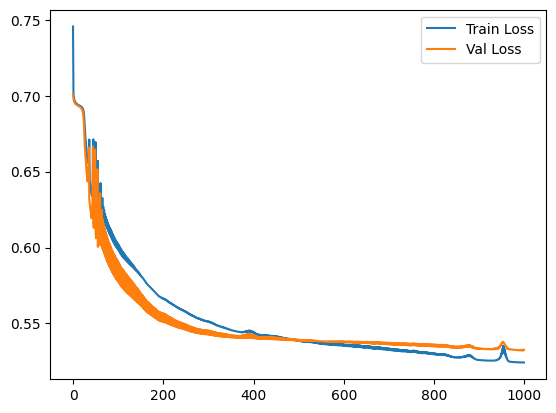
\includegraphics[width=0.75\textwidth]{ysa.png}
    \caption{Train ve Validation Loss Grafiği}
    \label{fig:my_pic}
\end{figure}
\newpage


\subsection{(10 Puan)} \textbf{SEED=öğrenci numaranız set ettikten sonra altıncı haftada ödev olarak verdiğim gibi earlystopping'deki en iyi modeli kullanarak, Prensesi İyileştir test setinden accuracy, F1, precision ve recall değerlerini hesaplayan kodu yazın ve sonucu da aşağı yapıştırın. \%80'den fazla başarı bekliyorum test setinden. Daha düşükse başarı oranınız, nerede hata yaptığınızı bulmaya çalışın. \%90'dan fazla başarı almak mümkün (ben denedim).}

\begin{python}
import torch
import torch.nn as nn
import torch.optim as optim
import pandas as pd
from sklearn.model_selection import train_test_split
import matplotlib.pyplot as plt
from sklearn.metrics import precision_recall_fscore_support
import copy

torch.manual_seed(190401035)

class MLP(nn.Module):
    def __init__(self, input_size, hidden_size1, hidden_size2, output_size):
        super(MLP, self).__init__()
        torch.manual_seed(1)
        self.fc1 = nn.Linear(input_size, hidden_size1)
        self.relu1 = nn.ReLU()
        self.fc2 = nn.Linear(hidden_size1, hidden_size2)
        self.relu2 = nn.ReLU()
        self.fc3 = nn.Linear(hidden_size2, output_size)
        self.sigmoid = nn.Sigmoid()

    def forward(self, x):
        out = self.fc1(x)
        out = self.relu1(out)
        out = self.fc2(out)
        out = self.relu2(out)
        out = self.fc3(out)
        out = self.sigmoid(out)
        return out


train_data = pd.read_csv('sample_data/cure_the_princess_train.csv')
val_data = pd.read_csv('sample_data/cure_the_princess_validation.csv')
test_data = pd.read_csv('sample_data/cure_the_princess_test.csv')


x_train = torch.tensor(train_data.iloc[:, :-1].values, dtype=torch.float)
y_train = torch.tensor(train_data.iloc[:, -1].values, dtype=torch.float).unsqueeze(1)
x_val = torch.tensor(val_data.iloc[:, :-1].values, dtype=torch.float)
y_val = torch.tensor(val_data.iloc[:, -1].values, dtype=torch.float).unsqueeze(1)
x_test = torch.tensor(test_data.iloc[:, :-1].values, dtype=torch.float)
y_test = torch.tensor(test_data.iloc[:, -1].values, dtype=torch.float).unsqueeze(1)

batch_size = 16

input_size = x_train.shape[1]
hidden_size1 = 100
hidden_size2 = 50
output_size = 1
model = MLP(input_size, hidden_size1, hidden_size2, output_size)
criterion = nn.BCEWithLogitsLoss()

optimizer = optim.SGD(model.parameters(), lr=0.1)


num_epochs = 1000
train_losses = []
val_losses = []
test_losses = []
train_accs = []
val_accs = []
test_accs = []

patience = 20
best_val_loss = float('inf')
counter = 0
best_model = None

for epoch in range(num_epochs):
    
    model.train()
    
    
    y_pred_train = model(x_train)
    train_loss = criterion(y_pred_train, y_train)
    train_losses.append(train_loss.item())

    
    optimizer.zero_grad()
    train_loss.backward()
    optimizer.step()

    
    model.eval()
    
    
    with torch.no_grad():
        train_acc = ((y_pred_train > 0.5).float() == y_train).float().mean()
        train_accs.append(train_acc.item())

    
    with torch.no_grad():
        y_pred_val = model(x_val)
        val_loss = criterion(y_pred_val, y_val)
        val_losses.append(val_loss.item())
        val_acc = ((y_pred_val > 0.5).float() == y_val).float().mean()
        val_accs.append(val_acc.item())

    
    with torch.no_grad():
        y_pred_test = model(x_test)
        test_loss = criterion(y_pred_test, y_test)
        test_losses.append(test_loss.item())
        test_acc = ((y_pred_test > 0.5).float() == y_test).float().mean()
        test_accs.append(test_acc.item())

    if val_loss.item() < best_val_loss:
        best_val_loss = val_loss.item()
        best_model = copy.deepcopy(model)
        counter = 0
    else:
        counter += 1

    if counter >= patience:
        print(f"Early stopping after {patience} epochs without improvement.")
        break

    if epoch % 100 == 0:
      print(f"Epoch {epoch}, Train Loss: {train_loss.item():.4f}, Val Loss: {val_loss.item():.4f}, Test Loss: {test_loss.item():.4f}, Test Acc: {test_acc:.4f}, Train Acc: {train_acc:.4f}, Val Acc: {val_acc:.4f}")

    

    with torch.no_grad():
      y_pred_train_bin = (model(x_train) > 0.5).float().numpy()
      y_pred_val_bin = (model(x_val) > 0.5).float().numpy()
      y_pred_test_bin = (model(x_test) > 0.5).float().numpy()

model = best_model
model.eval()

precision_train, recall_train, f1_train, _ = precision_recall_fscore_support(y_train.numpy(), y_pred_train_bin, average='binary')
precision_val, recall_val, f1_val, _ = precision_recall_fscore_support(y_val.numpy(), y_pred_val_bin, average='binary')
precision_test, recall_test, f1_test, _ = precision_recall_fscore_support(y_test.numpy(), y_pred_test_bin, average='binary')
        


print(f"Train - Precision: {precision_train:.4f}, Recall: {recall_train:.4f}, F1 Score: {f1_train:.4f}")
print(f"Val - Precision: {precision_val:.4f}, Recall: {recall_val:.4f}, F1 Score: {f1_val:.4f}")
print(f"Test - Precision: {precision_test:.4f}, Recall: {recall_test:.4f}, F1 Score: {f1_test:.4f}")

\end{python}

Epoch 0, Train Loss: 0.7456, Val Loss: 0.7007, Test Loss: 0.6982, Test Acc: 0.4974, Train Acc: 0.4417, Val Acc: 0.5032

Epoch 100, Train Loss: 0.5985, Val Loss: 0.5909, Test Loss: 0.6043, Test Acc: 0.7422, Train Acc: 0.8450, Val Acc: 0.7739

Epoch 200, Train Loss: 0.5663, Val Loss: 0.5566, Test Loss: 0.5663, Test Acc: 0.8562, Train Acc: 0.8962, Val Acc: 0.8694

Epoch 300, Train Loss: 0.5511, Val Loss: 0.5453, Test Loss: 0.5500, Test Acc: 0.8912, Train Acc: 0.9233, Val Acc: 0.9045

Early stopping after 20 epochs without improvement.

Train - Precision: 0.9640, Recall: 0.8687, F1 Score: 0.9139

Val - Precision: 0.9562, Recall: 0.8397, F1 Score: 0.8942

Test - Precision: 0.9758, Recall: 0.8299, F1 Score: 0.8969


\subsection{(5 Puan)} \textbf{Tüm kodların CPU'da çalışması ne kadar sürüyor hesaplayın. Sonra to device yöntemini kullanarak modeli ve verileri GPU'ya atıp kodu bir de böyle çalıştırın ve ne kadar sürdüğünü hesaplayın. Süreleri aşağıdaki tabloya koyun. GPU için Google Colab ya da Kaggle'ı kullanabilirsiniz, iki ortam da her hafta saatlerce GPU hakkı veriyor.}

\begin{table}[ht!]
    \centering
    \caption{Buraya bir açıklama yazın}
    \begin{tabular}{c|c}
        Ortam & Süre (saniye) \\\hline
        CPU & 2.4854421615600586 \\
        GPU & 2.9396817684173584\\
    \end{tabular}
    \label{tab:my_table}
\end{table}

\subsection{(3 Puan)} \textbf{Modelin eğitim setine overfit etmesi için elinizden geldiği kadar kodu gereken şekilde değiştirin, validasyon loss'unun açıkça yükselmeye başladığı, training ve validation loss'ları içeren figürü aşağı koyun ve overfit için yaptığınız değişiklikleri aşağı yazın. Overfit, tam bir çanak gibi olmalı ve yükselmeli. Ona göre parametrelerle oynayın.}

Cevaplar buraya

% Figür aşağı
\begin{comment}
\begin{figure}[ht!]
    \centering
    \includegraphics[width=0.75\textwidth]{mypicturehere.png}
    \caption{Buraya açıklama yazın}
    \label{fig:my_pic}
\end{figure}
\end{comment}

\subsection{(2 Puan)} \textbf{Beşinci soruya ait tüm kodların ve cevapların olduğu jupyter notebook'un Github linkini aşağıdaki url'e koyun.}

\url{https://github.com/aybukekcr/MultilayerPerceptron}

\section{(Toplam 10 Puan)} \textbf{Bir önceki sorudaki Prensesi İyileştir problemindeki yapay sinir ağınıza seçtiğiniz herhangi iki farklı regülarizasyon yöntemi ekleyin ve aşağıdaki soruları cevaplayın.} 

\subsection{(2 puan)} \textbf{Kodlarda regülarizasyon eklediğiniz kısımları aşağı koyun:} 

\begin{python}
kod_buraya = None
if kod_buraya:
    devam_ise_buraya = 0

print(devam_ise_buraya)
\end{python}

\subsection{(2 puan)} \textbf{Test setinden yeni accuracy, F1, precision ve recall değerlerini hesaplayıp aşağı koyun:}

Sonuçlar buraya.

\subsection{(5 puan)} \textbf{Regülarizasyon yöntemi seçimlerinizin sebeplerini ve sonuçlara etkisini yorumlayın:}

Yorumlar buraya.

\subsection{(1 puan)} \textbf{Sonucun github linkini  aşağıya koyun:}

\url{www.benimgithublinkim2.com}

\end{document}